\subsection{Define \texorpdfstring{$K_5$}{} and \texorpdfstring{$K_{3,3}$}{}}

\begin{center}
    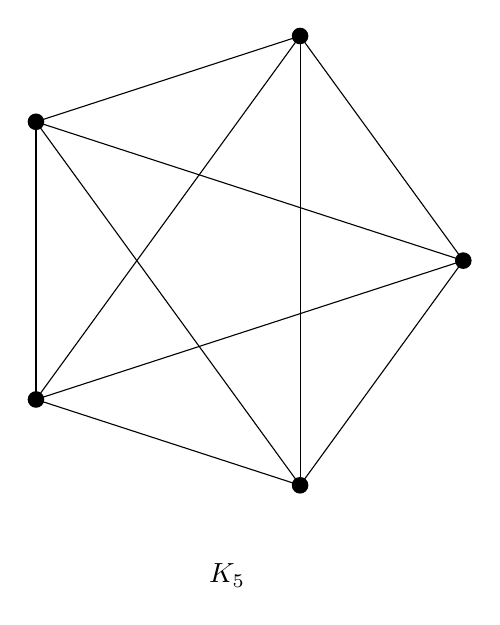
\begin{tikzpicture}
        \foreach \i in {1, 2, 3, 4, 5}
        \fill[black] (\i*360/5:3) coordinate (5\i) circle(3 pt)
        \ifnum \i>1 foreach \j in {\i,...,1}{(5\i) edge (5\j)} \fi;

        \node at (0,-4,0) {$K_5$};
    \end{tikzpicture}
    \hspace{2cm}
    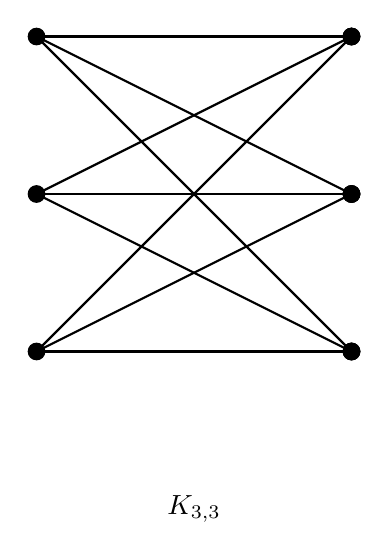
\begin{tikzpicture}
        \foreach \x/\y in {0/1, 0/3, 0/5} {
                \filldraw[black] (\x,\y) circle (3pt);
                \foreach \z/\t in {4/1, 4/3, 4/5} {
                        \filldraw[black] (\z,\t) circle (3pt);
                        \draw[black, thick] (\x,\y) -- (\z,\t);
                    }
            }
        \node at (2,-1,0) {$K_{3,3}$};
    \end{tikzpicture}
\end{center}